
\textbf{Introduction}\\
Dans ce chapitre nous allons préparer notre planification de projet ou «sprint 0». Cette phase représente une phase importante dans le cycle de développement SCRUM puisqu’elle a une influence directe sur la
réussite des sprints et en particulier le premier.
Nous allons spécifier en premier lieu les différents besoins fonctionnels et non fonctionnels, après nous allons fournir les éléments nécessaires afin de piloter le projet avec la méthode SCRUM. Enfin, nous allons présenter notre environnement de travail matériel et logiciel et l'architecture logique et physique de notre système.   
\section{Spécification des besoins}
Cette partie sert à identifier les fonctionnalités attendues dans l’application. Elle résume les besoins fonctionnels auxquels doit répondre l’application.

\subsection{Les besoins fonctionnels}
Le Centre National Universitaire de documentation Scientifique et Technique (CNUDST)
souhaite automatiser la gestion des formations qu’il organise périodiquement au profit de
la communauté scientifique tunisienne.\\
On peut distinguer trois types de formations qui sont:
\begin{enumerate}
	\item Les ateliers
	\item Les workshops avec éditeurs : sont assurés par les éditeurs de revues, ouvrages ou bases de données scientifiques
	\item Les journées d’information sur les ressources électroniques
\end{enumerate}

Les ateliers: assurés par le personnel du CNUDST portent sur 3 thèmes bien
déterminés à savoir :
\begin{enumerate}
	\item Méthodologie de la recherche bibliographique,
	\item Utilisation des outils de référencement bibliographique : cas de Endnote,
	\item Utilisation des outils bibliographiques et bibliométriques.
	Ces ateliers subdivisent en deux catégories : 
	
\end{enumerate}
Ces ateliers peuvent être publics et gratuits, animés dans les locaux du CNUDST en général au mois de Janvier ou des ateliers ciblés, payants et sur demande des
institutions.\\
La participation aux ateliers gratuits dans les locaux du CNUDST se fait à travers
une préinscription réalisée en ligne. Le processus d’inscription à
ces ateliers se déroule selon les étapes suivantes :
\\
\underline{\textit{Etape1 : Préinscription :}}\\
Un formulaire de préinscription est publié par le CNUDST sur son site
web, pendant une période bien déterminée.\\
L’annonce et l’ouverture des préinscriptions se font en même temps et englobent au
départ toutes les sessions des thèmes.\\
La fermeture de la préinscription se fait sur demande du formateur concerné et
par session, selon le nombre de demandes d’inscription reçues et le nombre de
places disponibles pour chaque session.\\
Le lien devient inaccessible dès que toutes les sessions seront comblées.\\ 
\underline{\textit{Etape 2 : Sélection des préinscriptions :}}\\
La sélection des préinscriptions se fait en se basant sur des critères fixés par
chaque formateur, parmi ces critères :
\begin{itemize}
	\item Le nombre de places (limité).
	\item La qualité de la personne préinscrite (par exemple un chercheur a la
	priorité par rapport à un étudiant, un bibliothécaire ne peut pas assister à
	ce genre d'ateliers, …).
	\item Une seule préinscription par session et par thème est retenue (les
	préinscriptions redondantes, pour le même thème sur des sessions
	différentes, seront rejetées).
\end{itemize}
\underline{\textit{Etape 3 : Demande de confirmation des inscriptions :}}\\
Une demande de confirmation de l’inscription est envoyée à la liste des personnes
sélectionnées pour assister à la formation.\\
Cette liste contient un nombre
supérieur à celui des places disponibles (en moyenne, 10 places) pour combler les
éventuelles absences d’un ou plusieurs participants).\\
\underline{\textit{Etape 4 : Approbation des inscriptions :}}\\
Une liste finale des inscrits est fixée et un e-mail de confirmation des inscriptions
est envoyé aux personnes concernées avec les détails suivants :
\begin{itemize}
	\item Date, heure et lieu de formation
	\item Outils de travail
\end{itemize}
Un atelier payant est organisé à la suite d’une demande issue de la part d’une institution
universitaire ou de recherche ou un établissement privé.\\
Le lieu de la formation et les outils matériels et techniques nécessaires pour le bon
déroulement de la formation sont à la charge du demandeur de la formation.\\ Ces ateliers
portent sur les mêmes thèmes que les ateliers gratuits.\\
Le processus de déroulement de ce type de formation est le suivant :\\
\underline{\textit{Etape1: Réception d’une demande de formation}}\\
Le CNUDST reçoit une correspondance, au nom du directeur général,
ayant pour objet une demande de formation.\\
\underline{\textit{Etape2: Traitement de la demande:}}\\
La demande sera remise au responsable de l’organisation des formations pour la
traiter:
\begin{itemize}
	\item Si la correspondance ne contient pas les informations nécessaires, le responsable
	de l’organisation des formations envoie une nouvelle correspondance, à travers la
	direction générale, dans
	laquelle il sera demandé de fournir plus d’informations sur la demande tout en
	mentionnant : les thèmes de formations, les tarifs, le nombre maximum de
	personnes qui peuvent assister (avec une copie de l’arrêté du 13 Février 2017
	fixant les tarifs des services payants rendus par le CNUDST). 
	\item Si la correspondance contient les informations nécessaires, le responsable de
	l’organisation des formations commence le traitement de la demande en
	collaboration avec l’équipe des formateurs (disponibilité des dates et des
	formateurs).
\end{itemize}
\underline{\textit{Etape2: Traitement de la demande:}}\\
Une correspondance est envoyée au demandeur de la formation en vue de confirmation de
la demande de formation et de transmission de participants (Nom
et Prénom) pour préparer les attestations. Cette correspondance contient les
informations suivantes :
\begin{itemize}
	\item Le ou les thèmes de formation.
	\item Les dates de formations.
	\item La liste des formateurs.
	\item Le programme des formations.
\end{itemize}
\underline{\textit{Etape 4 : Confirmation de la formation}}\\	
Réception d’une confirmation envoyée par le représentant du
demandeur de la formation.


\subsection{Les besoins non fonctionnels}
Les besoins non fonctionnels caractérisent le système et affectent le flux réel de l'application. Ce sont des besoins techniques qui décrivent la plupart des contraintes auxquelles le système est soumis et qui permet d'assurer sa mise en oeuvre et son bon fonctionnement.
Dans ce cas notre projet doit respecter un ensemble de besoins pour avoir une meilleure performance telles que:
\begin{itemize}
	\item \textbf{La Fiabilité :}\\
	Cette exigence veut dire que notre application doit effectuer les fonctionnalités prévues dans les
	conditions normales d’utilisations. C’est-à-dire dans le cas où il n'y a aucune exception, notre application
	doit accomplir sa mission.
	\item \textbf{La Portabilité :}\\
	Notre application doit être compatible avec n’importe quel système d’exploitation.
	\item \textbf{L'Ergonomie:}\\
	Les interfaces de notre solution doivent être ergonomiques et conviviales, elles doivent être aussi  lisible et facile à manipuler par n'importe quel utilisateur sans difficultés.
	\item \textbf{L'Extensibilité :}\\
    Notre application doit adopter une implémentation claire et simple et un code lisible pour permettre en cas de
	besoin, une modification facile des fonctionnalités existantes ainsi que l’ajout des nouvelles
	fonctions.
	\item \textbf{La Performance:}\\Au niveau du temps de réponse, nous allons veiller, aussi, à ce que notre site ait un temps de
	réponse rapide pour garantir la fluidité de navigation et une expérience utilisateur de qualité. Nous
	proposons d’évaluer la performance (rapidité) avec le service en ligne PageSpeed :
	https://pagespeed.web.dev/
	\item \textbf{La Compatibilité}\\
	Notre site web est développé avec les technologies récentes et il est compatible avec la plupart
	des navigateurs du marché :
	\begin{itemize}
		\item Navigateurs desktop: Google Chrome, Mozilla Firefox, Microsoft Edge, Opera, Safari. 
		\item Navigateurs mobile: Chrome, Firefox, Opera, Samsung Internet, UC Browser, Brave Browser…
		
	\end{itemize}
	
	Nous allons tester la compatibilité de note application avec le navigateur le plus populaire
	avec le service en ligne BowserLing sur le site : \\https://www.browserling.com/
	\item \textbf{La Sécurité:}\\
	La sécurité générale de notre site est assurée par un backup automatisé pour
	sauvegarder les données. Le développement de notre site est effectué tout en respectant
	le guide de test de sécurité Web OWASP.\\
	Notre site garantit la sécurité des données personnelles :
	\begin{itemize}
		\item Exigences à respecter au niveau du remplissage du formulaire,
		\item Validation de tous les champs,
		\item Gestion des droits d’accès,
		\item Protection contre les spam et les abus avec le service reCAPTCHA de Google,
	\end{itemize}
\end{itemize}
\section{Modélisation des besoins}
Les diagrammes de notre application sont effectués grâce à l'outil de conception graphique \textbf{draw.io}.
Il est disponible en ligne sur le lien suivant:\url{https://www.diagram.net}.\\
Le diagramme de cas d'utilisation de notre système est représenté comme suit:
%\newpage
\begin{figure}[!h]
	\centering
	{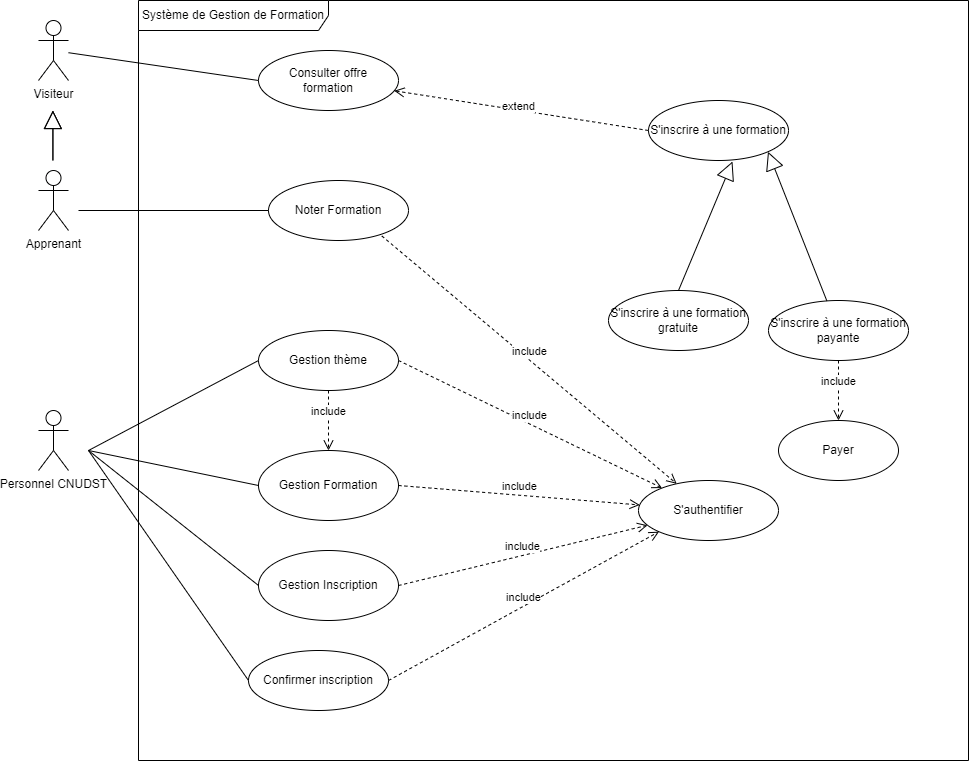
\includegraphics[width=1\textwidth]{D) IMAGES/casutlglobal.png}}
	\caption{Diagramme des cas d'utilisation globale du système}
	\label{Diagramme3}
\end{figure}

\section{Pilotage du projet avec SCRUM}
\subsection{Rôles de SCRUM}
\begin{table}[!h]
	\centering % used for centering table
	\begin{tabular}{ |c|c| } 
		
		
		\hline% inserts single horizontal line
		\centering{\textbf{~~~~Rôle SCRUM~~~~}} & \textbf{~~~~Personnes Affectées~~~~} \\
		\hline
		Product Owner & Chokri Ben Romdhane\\ 
		\hline  
		SCRUM Master & Bassem Boughzala   \\ 
		\hline
		Developpers Team & Olfa Chaouech  \\
		\hline
		
		
		
	\end{tabular}
	
	\caption{équipe et rôles Scrum}
\end{table}
\section{Backlog du produit}
Le tableau ci-dessous présente le « Backlog » du produit initial. Le « Backlog » se traduit par un
ensemble de «user stories» qui décrivent les fonctionnalités attendues de l’application.\\
A chaque «user story» est associé un identifiant et une priorité.\\
Une ou plusieurs user stories peuvent être regroupées dans un EPIC.
\begin{table}[!h]
	\centering % used for centering table
	\begin{tabular}{|p{4cm}|p{1cm}|p{8.5cm}|c|}
		\hline
		\textbf{EPIC}&\textbf{Id} & \centering{\textbf{User Story}} & \textbf{Priorité}\tabularnewline
		\hline
		& US1  & En tant qu'administrateur, je peux créer un thème &1\\
		\cline{2-4}
		& US2  & En tant qu'utilisateur, je peux consulter la liste des thèmes (All Events) &2\\
		\cline{2-4}
		\multirow{-2}{2cm}{Gestion thème de formation}& US3&En tant qu'administrateur, je peux mettre à jour un thème de formation & 3\\
		\cline{2-4}
		& US4  & En tant qu'utilisateur, je peux consulter les détails d'un thème&4\\
		\cline{2-4}
		\hline
		
		& US5  & En tant qu'administrateur, je peux intégrer des formations dans le thème&5\\
		\cline{2-4}
		\multirow{-2}{2cm}{Gestion formation}& US6&En tant qu'administrateur, je peux mettre à jour une  formation & 6\\
		\hline
		& US7  & En tant qu'utilisateur je peux consulter la liste des
		formations&7\\
		\cline{2-4}
		& US8&En tant qu'utilisateur je peux consulter les détails des
		formations& 8\\
		\cline{2-4}
		\multirow{-3}{3cm}{Consultation des offres de formation}& US9  & 
		En tant qu'utilisateur je veux contacter les responsables du site
		pour avoir plus d’informations sur une offre&9\\
		\hline
		
	& US10&En tant qu'utlisateur je veux m’inscrire pour pouvoir participer à une formation & 10\\
		\cline{2-4}
			\multirow{-2}{4cm}{Inscription à une Formation en ligne}& US11&En tant qu'administrateur ou apprenant, je veux m'authentifier & 11\\
			\cline{2-4}
	& US12&En tant qu'administrateur, je peux confirmer une inscription& 12\\
	
		
			
		\hline
	& US13&En tant qu'apprenant, je veux donner mon avis concernant une formation & 13\\
	\cline{2-4}
	\multirow{-2}{4cm}{Interaction sur le site}& US14&En tant qu'administrateur ou apprenant, je peux modifier une note concernant une formation  & 14\\
	\cline{2-4}
	& US15&En tant qu'administrateur ou apprenant, je peux Supprimer une note concernant une formation  & 15\\
	\hline	
		
	\end{tabular}
	\caption{Tableau : Backlog product}
\end{table}

\section{La planification de release}
La planification de release fournit des informations sur le contenu des sprints, dans le cas de notre
projet, la réalisation de l’application nécessite une release qui commence le $02/05/2022$ et se termine le $02/09/2022$.
\subsection{Durée des sprints}
Après l’estimation de nos « user stories », nous avons partagé notre release sur trois sprints d’une
durée de quatre semaines.
\subsection{Planning des sprints}
Voici la répartition temporelle des trois sprints que nous allons réaliser dans les chapitres suivants.
\begin{figure}[!h]
	\centering
	{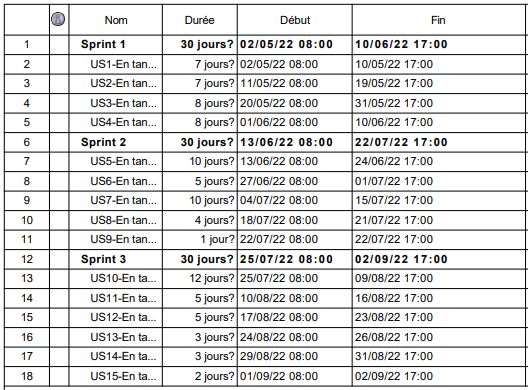
\includegraphics[width=0.95\textwidth]{D) IMAGES/PlanningdesSprints.png}}
	\caption{Planning des sprints-feuille de calcul (ProjectLibre)}
	\label{Org}
\end{figure}
\begin{figure}[!h]
	\centering
	{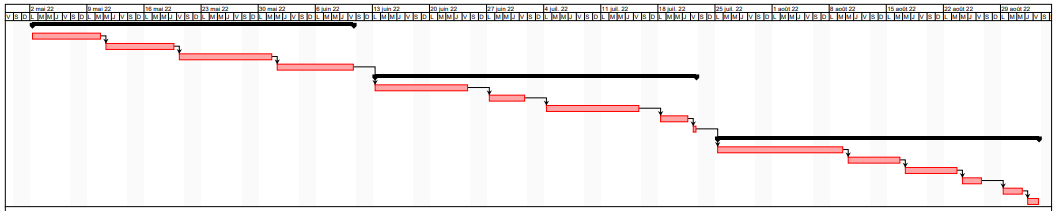
\includegraphics[width=0.95\textwidth]{D) IMAGES/PlanningDesSprintsGantt.png}}
	\caption{Planning des sprints-diagramme de Gantt (ProjectLibre)}
	\label{Org}
\end{figure}
\section{Environnement de travail}
\subsection{Environnement matériel}
Nous présentons les caractéristiques de nos outils matériels utilisés pour la réalisation de notre application.
\begin{table}[!h]
	\centering % used for centering table
	\begin{tabular}{ |c|p{10cm}| } 
		
		
		\hline% inserts single horizontal line
		\centering{\textbf{Type}} & \textbf{~~~~~~Désignation} \\
		\hline
	Marque & ASUS\\ 
		\hline  
		Processeur & Intel(R) Core(TM):7-106567 CPU@1.30 GHZ 1.50 GHZ   \\ 
		\hline
		RAM & 20 GO  \\
		\hline
	Système d'exploitation & Windows 10 \\ 
		
		\hline 
		Architecture & 64 bit \\
		\hline
		
	\end{tabular}
	\begin{flushright}
		\footnotesize Source: Digital guide ionos: Comparatif de CMS 2022 .\end{flushright}
	\caption{Caractéristiques de l'Environnement Matériel}
\end{table}
\subsection{Environnement logiciel}
\begin{enumerate}
	\item Outils de développement et modélisation
	\begin{itemize}
		\item Pour le développement, nous avons utilisé : \textbf{VSCode} et\textbf{WAMP}.
		\item Pour la modélisation, nous avons utilisé: \textbf{draw.io}
	\end{itemize}
	\item Langage de programmation et framework\\
	Les langages et framework de programmation que nous avons utilisés.
	\begin{itemize}
		\item \textbf{Côté front-end}
		\begin{itemize}
			\item HTML, CSS et JavaScript.
		\end{itemize}
		\item \textbf{Côté back-end}
		\begin{itemize}
			\item Langage php,
			\item Rest API,
			\item MySQL , 
		\end{itemize}
    	\item \textbf{Logiciel de gestion de projet Scrum}\\
    	Pour la gestion du projet par la méthode SCRUM, nous avons utilisé: Trello et Project Libre.
		\item \textbf{Côté hébergement et déploiement}
		\begin{itemize}
			\item Github.git
			\item Latex
		\end{itemize}
		
	\end{itemize}
\end{enumerate}
\subsection{Présentation des logiciels et outils utilisés}
	
	\begin{itemize}
		\item  \begin{minipage}{.10\textwidth}%
			
\includegraphics[width=0.95\textwidth]{D) IMAGES/html.png}
		\end{minipage}%
		L’HyperText Mark up Langage, généralement abrégé HTML, est le langage de balisage conçu pour représenter les pages web.
C’est un langage permettant d’écrire de l’hypertexte, d’où son nom. HTML permet également de structurer sémantiquement et logiquement et de mettre en forme le contenu des pages, d’inclure des ressources multimédias dont des images, des formulaires de saisie et des éléments 
programmables tels que des applets. 
	\item \begin{minipage}{.10\textwidth}%
		
\includegraphics[width=0.95\textwidth]{D) IMAGES/css.png}
	\end{minipage}%	
Les feuilles de style en cascade, généralement appelées CSS de l'anglais Cascading Style Sheets, forment un langage informatique qui décrit la présentation des documents HTML et XML. Les standards définissant CSS sont publiés par le World Wide Web Consortium (W3C). Introduit au milieu des années 1990, CSS devient couramment utilisé dans la conception de sites web et bien pris en charge par les navigateurs web dans les années 2000 (Wikipédia,2019a et IWM,2020).
 \item \begin{minipage}{.15\textwidth}%
 	
\includegraphics[width=0.95\textwidth]{D) IMAGES/latex.jpg}
 \end{minipage}% 
\LaTeX est un langage informatique, un logiciel libre et un système de composition de document.\\
Ce système a été développé par le chercheur américain "Leslie Lamport". Il s'agit d'une version simplifiée du système Tex de "Donald Knuth".\\
Nous avons choisi \LaTeX  car il permet de rédiger des documents dont la mise en page est réalisée automatiquement en se conformant du mieux possible à des normes typographiques.\\
Le tableau suivant permet de comparer  \LaTeX~et Word.  

\begin{table}[ht]
	\centering
	\begin{tabular}{c|cc}
		\hline
		& Word, OpenOffice & \LaTeX   \\
		\hline
		\rowcolor{LightCyan}
		Apprentissage à court terme& Facile & Dur  \\
		Changement de la mise en page& Facile & Dur\\
		\rowcolor{LightCyan}
		Interaction avec le document& Direct & Indirect \\
		Fonctionnalités avancées& Includes & Par morceaux \\
		\rowcolor{LightCyan}
		Multi-plateforme& Non & Oui  \\
		Formules mathématiques& Récent & Très robuste  \\
		\rowcolor{LightCyan}
		Longévité de la compatibilité& Courte & Longue  \\
		Algorithme de mise en page& Pauvre & Evolué\\
		\rowcolor{LightCyan}
		Structuration du document & Optionnelle & Obligatoire \\
		Nombre de polices& Très élevé & Par morceaux \\
		\rowcolor{LightCyan}
		Bibliographie& Externe & Automatique  \\
		Edition avec ChemDraw & Directe & Indirecte  \\
		\rowcolor{LightCyan}
		Images inclues dans le fichier & Oui & Non \\
		Poids d'un fichier & $\approx$ 10 Mo & $\approx$ 500 Ko\\
		\hline
		
	\end{tabular}
	\caption{Comparaison Word /\LaTeX}
\end{table}


     
 	\item  \begin{minipage}{.10\textwidth}%
 		
\includegraphics[width=0.95\textwidth]{D) IMAGES/java.png}
 	\end{minipage}% 
 JavaScript : JavaScript est un langage de programmation de scripts principalement employé dans les pages web interactives mais aussi pour les serveurs avec l'utilisation, par exemple, de Node.js. C'est un langage orienté objet à prototype, c'est-à-dire que les bases du langage et ses principales interfaces sont fournies par des objets qui ne sont pas des instances de classes, mais qui sont chacun équipés de constructeurs permettant de créer leurs propriétés, et notamment une propriété de prototypage qui permet d'en créer des objets héritiers personnalisés.
 \item  \begin{minipage}{.15\textwidth}%
 	
\includegraphics[width=0.95\textwidth]{D) IMAGES/php.jpg}
 \end{minipage}% 
PHP: Hypertext Preprocessor, plus connu sous son sigle PHP (sigle auto-référentiel), est un langage de programmation libre, principalement utilisé pour produire des pages Web dynamiques via un serveur HTTP, mais pouvant également fonctionner comme n'importe quel langage interprété de façon locale. PHP est un langage impératif orienté objet.

PHP a permis de créer un grand nombre de sites web célèbres, comme Facebook et Wikipédia. Il est considéré comme une des bases de la création de sites web dits dynamiques mais également des applications web.(Wikipédia)\\
Le, CMS WordPress que nous avons utilisé pour le développement de notre interface web, est écrit avec le langage de script PHP.\\





\item  \begin{minipage}{.15\textwidth}%
	
\includegraphics[width=0.95\textwidth]{D) IMAGES/VSCode.png}
\end{minipage}% 
Visual Studio Code : est un éditeur de code open-source, gratuit et multi-plateforme (Windows, Mac et Linux), développé par Microsoft.
Visual Studio Code prend immédiatement en charge presque tous les principaux langages de programmation et de balisage. Plusieurs d'entre eux sont inclus par défaut, par exemple JavaScript, TypeScript, CSS et HTML, mais d'autres extensions de langage peuvent être trouvées et téléchargées gratuitement à partir de VS Code Marketplace.
\item \begin{minipage}{.25\textwidth}%
	
\includegraphics[width=0.95\textwidth]{D) IMAGES/draw.png}
\end{minipage}%
Pour la modélisation, nous avons utilisé "draw.io" connu aussi sous diagrams.net, il s'agit d'un outil de création de diagrammes gratuit et collaboratif.\\
Il permet aux utilisateurs de créer et de partager des diagrammes dans un navigateur web. 

 \item  \begin{minipage}{.25\textwidth}%
 	
\includegraphics[width=0.95\textwidth]{D) IMAGES/sql.png}
 \end{minipage}% 
C’est un logiciel de gestion et d’administration de base de données. Via une interface graphique 
intuitive, il permet de manipuler (créer, modifier supprimer) des objets, des données, des comptes 
utilisateurs, et d’effectuer toutes les opérations inhérentes à la gestion d’une base de données. Pour 
cela il doit être connecté à un serveur MySQL.
	
\end{itemize}
\section{Architecture de l'application}

\subsection{Architecture physique}
Nous allons choisir une architecture 3-tiers pour notre application. L’architecture à trois
couches est une architecture client-serveur adaptée aux applications web et permet :
\begin{itemize}
	\item Une plus grande flexibilité /souplesse,
	\item Une plus grande sécurité (la sécurité peut être définie pour chaque service),
	\item De meilleures performances (les tâches sont partagées).
\end{itemize}
\begin{figure}[!h]
	\centering
	{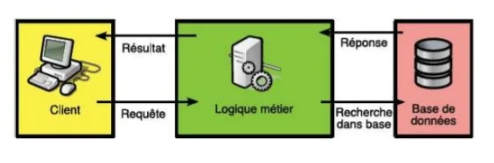
\includegraphics[width=0.85\textwidth]{D) IMAGES/arch.png}}
	\caption{Architecture physique 3-tiers}
	\label{Diagramme3}
\end{figure}
\subsection{Architecture logique}
La démarche MVC est un patron de conception qui sépare les données (le modèle), l’interface 
homme-machine (la vue) et la logique de contrôle(le contrôle).

\begin{figure}[!h]
	\centering
	{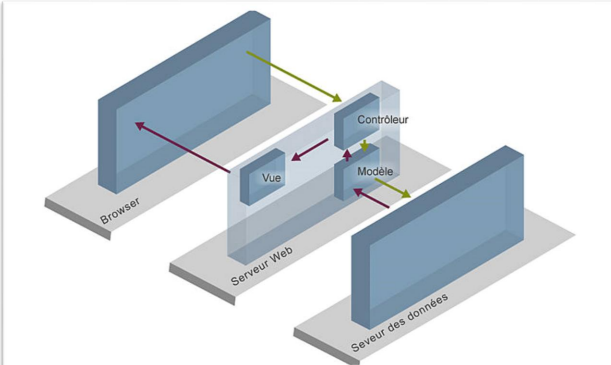
\includegraphics[width=0.65\textwidth]{D) IMAGES/MVC.png}}
	\caption{Architecture logique MVC}
	\label{Diagramme3}
\end{figure}

\begin{itemize}
	\item \textbf{Modèle} : Encapsule le cœur fonctionnel de l’application, le domaine logique.
	\item \textbf{Vue}:Les données sont envoyées par le modèle, à la vue qui les visualise à l’utilisateur.
	\item \textbf{Contrôleur}: Cet objet - car il s'agit aussi d'un objet - permet de faire le lien entre la vue et 
	le modèle lorsqu'une action utilisateur est intervenue sur la vue. C'est cet objet qui aura pour 
	rôle de contrôler les données.
	

\end{itemize}

\textbf{Conclusion}\\
A travers ce chapitre, nous avons spécifié les besoins fonctionnels et non fonctionnels de la solution en premier lieu. En second lieu, nous avons construit notre backlog du produit qui va nous permettre de bien entamer le premier sprint de notre projet que nous allons aborder dans le chapitre suivant.
